%\usepackage{cleveref}
\chapter{Results}

\label{ch:results}

\section{ATLAS\textsuperscript{3D}}
Initially, the algorithm was trained using the $\lambda_{Re}$ to predict the FS classification since they were related directly according to ref{eq:2.4}
(NEED TO FIX REFERENCING EQUATIONS). Promisingly, the classifier was 100\% successful in its predictions. Training was then performed using the Se\'rsic index of the single fit, n, and achieved success of 71\% which exactly matched the probability of randomly selecting the answer given by the binomial probability distribution which is necessary due to the binomial nature of the outcome with differing sizes of the two populations, given by\cite{simmons_2016}:
\begin{equation}
P(k,n) = \binom{n}{k}p^{k}q^{n-k}
\end{equation}
where $n$ is the number of trials, $k$ is the number of successes, $n-k$ is the number of failures, $p$ is the probability of success in one trial and $q=1-p$ is probability of failure in one trial. This indicates that the algorithm failed in its attempt to predict the rotation based on se\'rsic index alone. This is surprising given the morphological importance of this parameter, but maybe due to...\\
When we look at the D/T dependence of the $\lambda_{Re}$ value, we see a more promising separation of the two populations, with a value of D/T $\approx 0.28$ producing a low level of impurity. This parameter was identified as the most promising by \cite{Krajnovic2013}[p1790].
\begin{figure}[h]
	\centering
	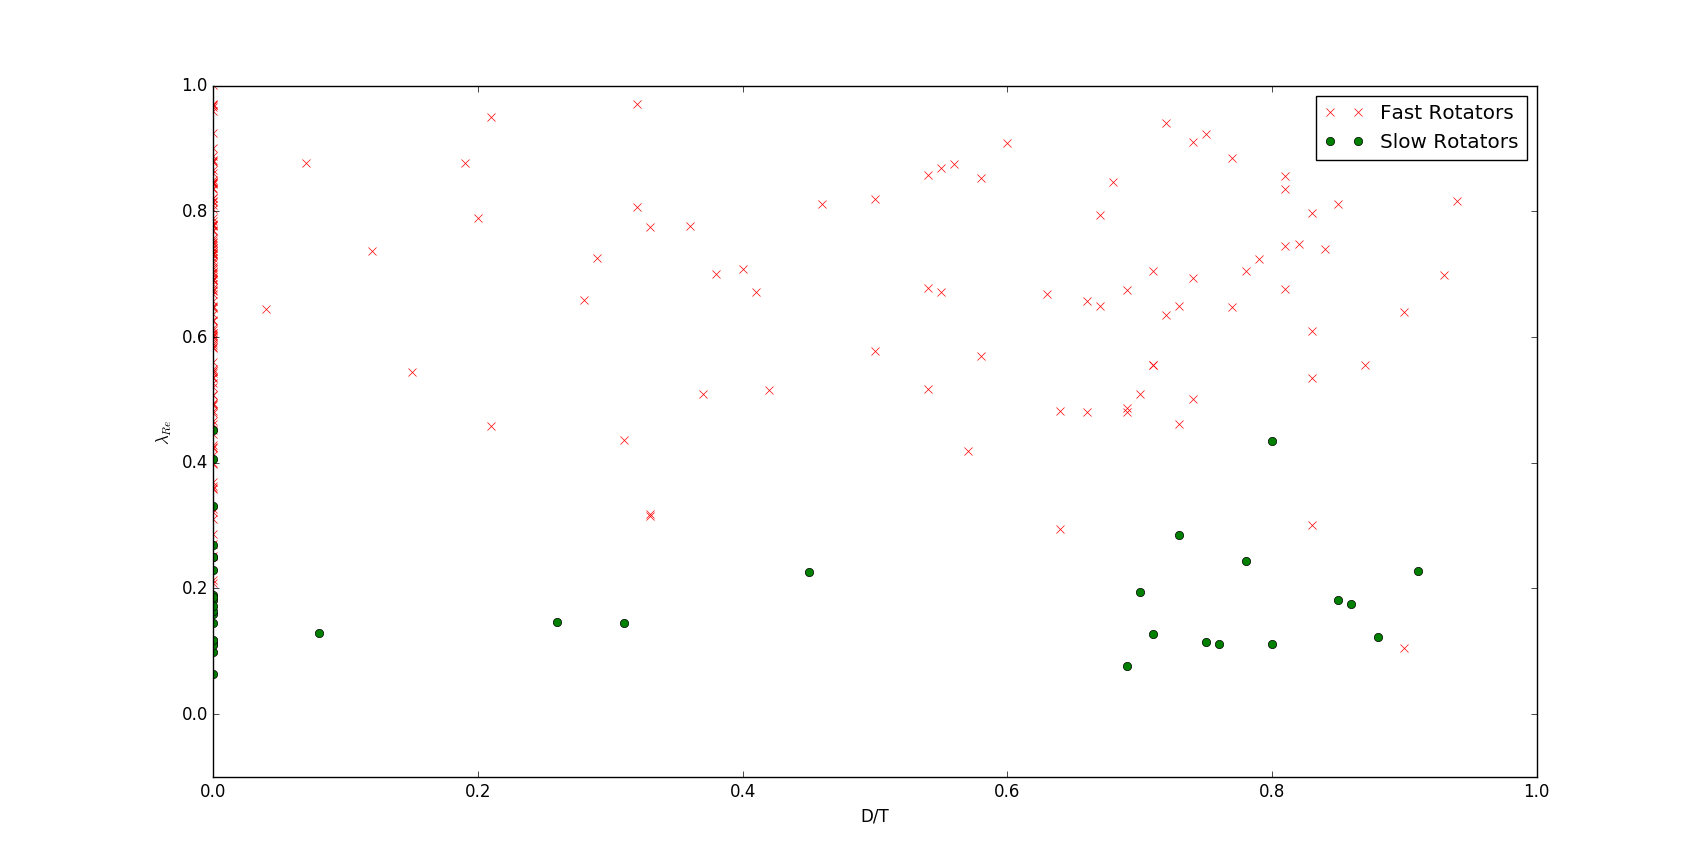
\includegraphics[width=\textwidth]{DT_lamre.png}
	\caption{The separation between the two populations is more pronounced here. The galaxies with D/T = 0 have no exponential discs.
	}
	\label{fig:dtlamre}
\end{figure}
The algorithm was then trained using D/T, improving the success rate to 81\%. Interestingly, when we evaluate the success of the decision tree classifier for those galaxies with no exponential disk component, where D/T$\lesssim $0.05, we find that the decision tree is still able to correctly classify the majority of galaxies.
\begin{figure}[h]
	\centering
	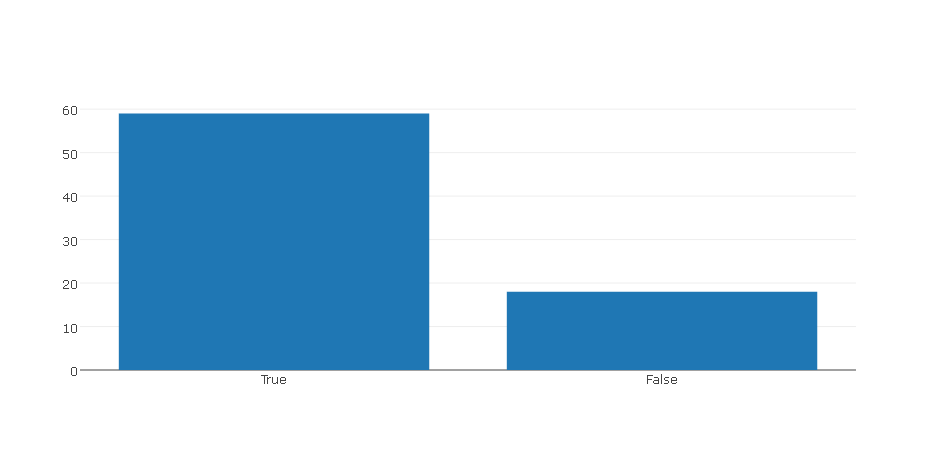
\includegraphics[width=\textwidth]{DTSuccessBar.png}
	\caption{Prediction success for galaxies with D/T $\lesssim$ 0.05.}
	\label{fig:dtbar}
\end{figure}
The success rate for just these galaxies is $\approx$77\% which is more than that expected from the binomial distribution. However, the apparent success is undermined when we plot the results for just these galaxies in \ref{zerodt}.
\begin{figure}[h]
	\centering
	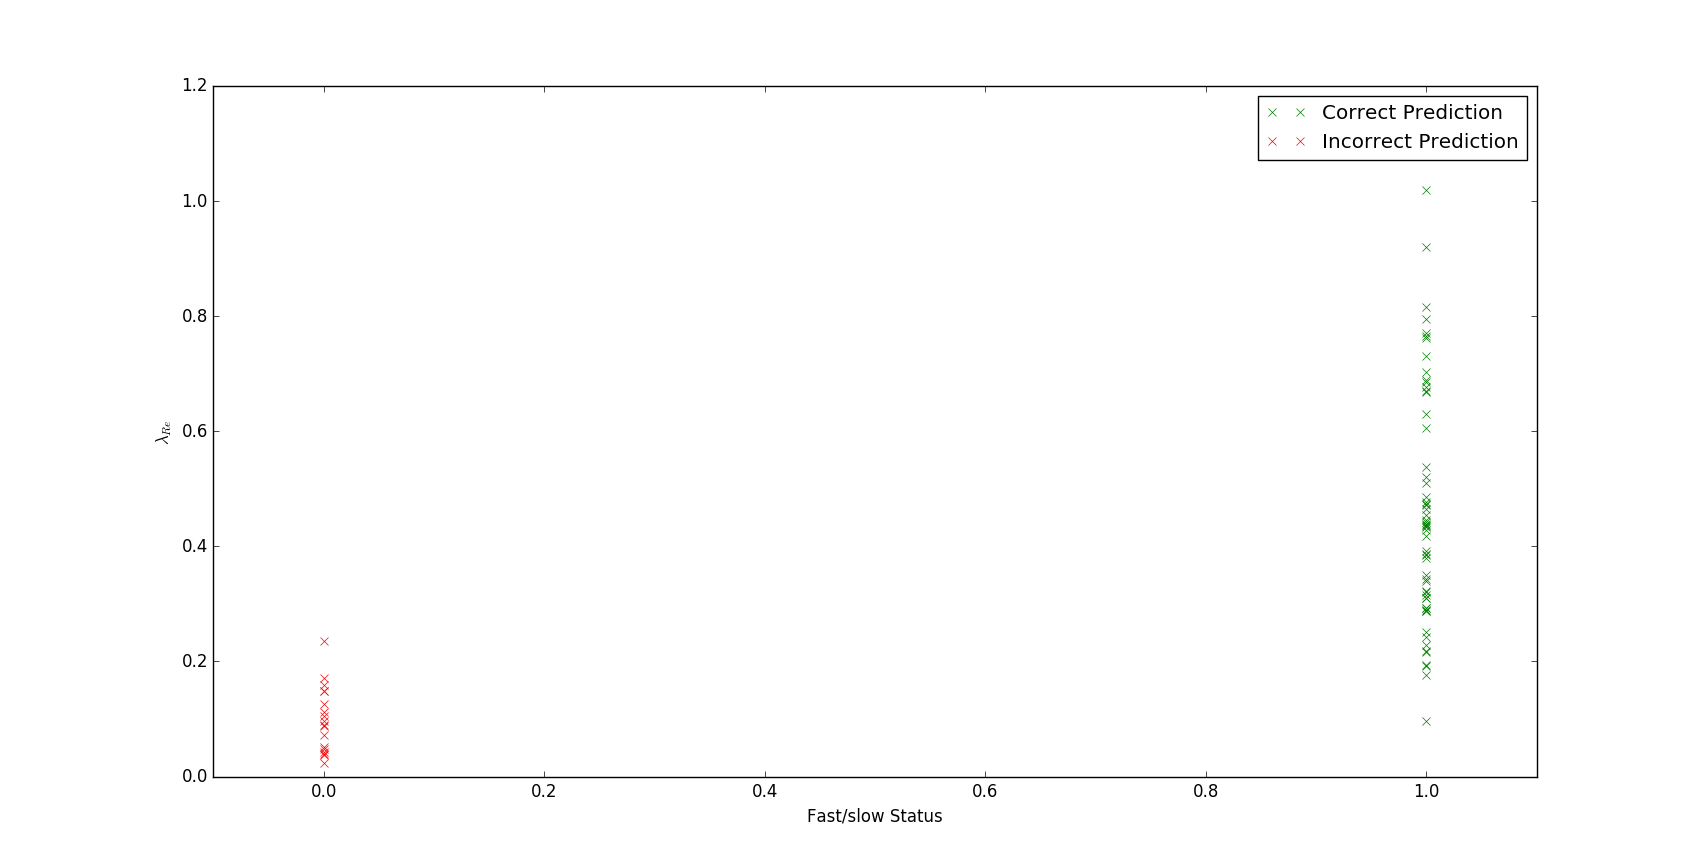
\includegraphics[width=\textwidth]{zerodt.png}
	\caption{Investigating the results where D/T$\lesssim $0.05. We see that the algorithm predicts galaxies to be universally fast rotators.
	}
	\label{fig:zerodt}
\end{figure}
The algorithm benefited from the fact that only $\approx$10\% of the galaxies with no disk in the test set were slow rotators. If the choice was made randomly, the success would be $\approx$15\%, and so represents a significant improvement, but would hardly require such statistical learning methods to make the conclusion that if there is no disk it is most likely a fast rotator.
The algorithm was then trained using both D/T and Se\'rsic index of the single fit by passing the features as an $n\times 2$ matrix, resulting in a success rate of 75\%, exceeding expectations based on random guess alone, but is less than what was achieved using D/T alone. The plots suggest that the algorithm is attempting to slow rotators more often rather than blindly assuming all galaxies are fast rotators, but it only successfully predicts a slow rotator once. Furthermore, 
\begin{figure}[h]
	\centering
	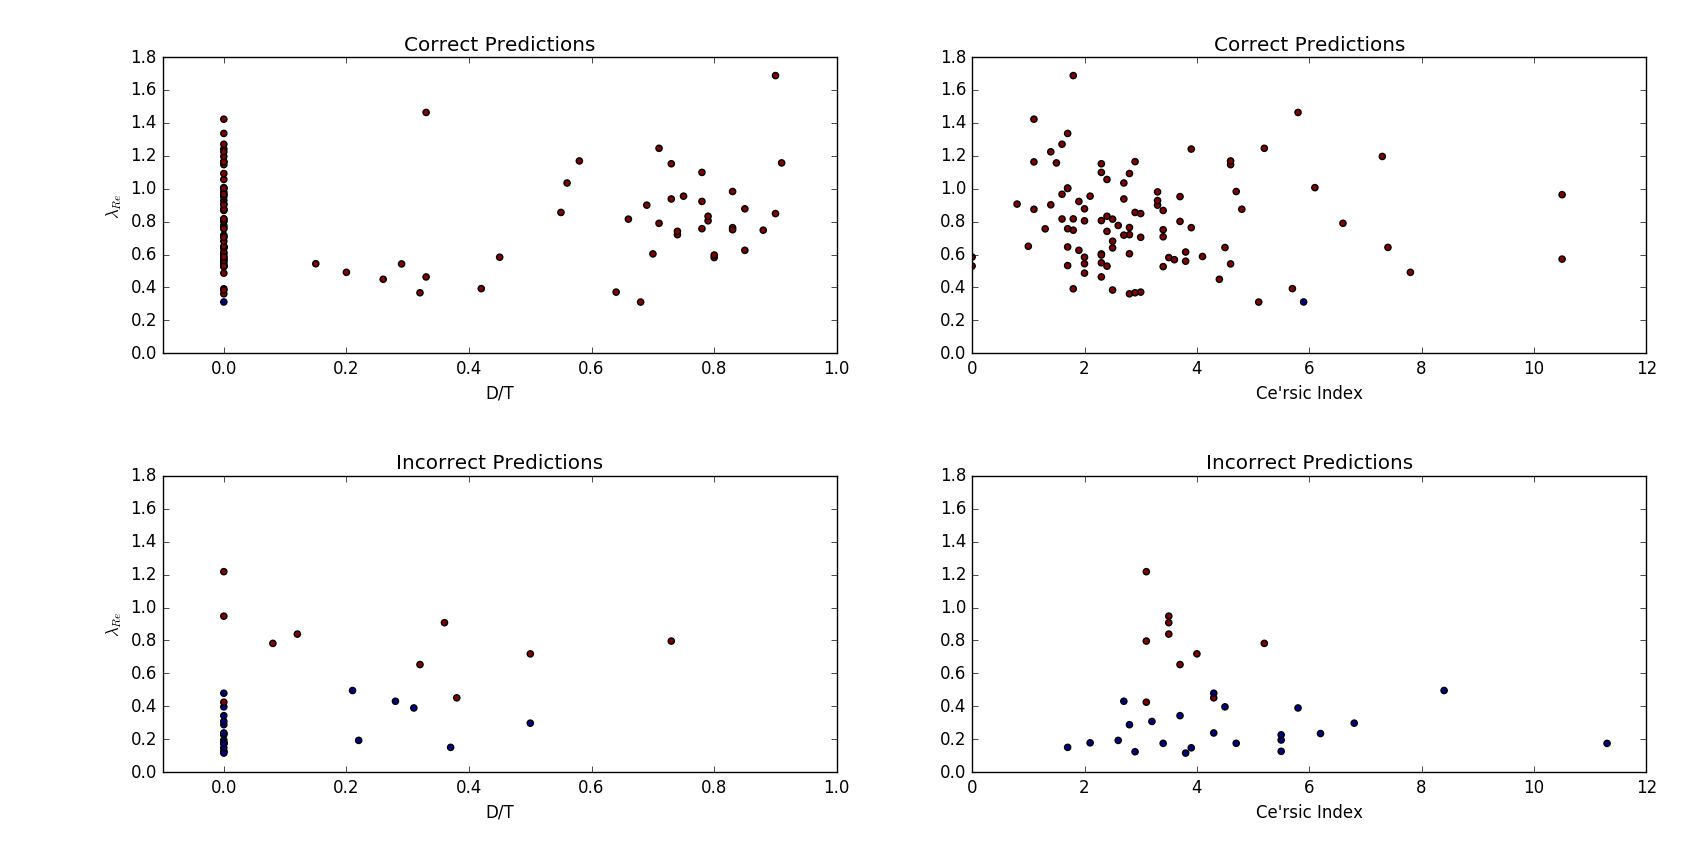
\includegraphics[width=\textwidth]{multiplot_correctincorrect_2d_withcol.png}
	\caption{Evaluating the success of decision trees with 2 variables, se\'rsic index and D/T. The markers are colour coded to be magenta for fast rotators and blue for slow rotators.
	}
	\label{fig:correctvsincorrect}